\documentclass[a4paper,12pt,titlepage]{article}
\usepackage[pdftex]{graphicx}
\usepackage[headheight=15pt]{geometry}

\usepackage{fancyhdr}
\pagestyle{fancy}
\lhead{Exercises}
\chead{}
\rhead{PostgreSQL / PostGIS}

\usepackage[english]{babel}									
\usepackage[utf8]{inputenc}	

\usepackage{array}
\usepackage{colortbl}

\usepackage{upquote}
\usepackage{listings}
\renewcommand{\lstlistlistingname}{List of Listings}
\lstset{language=SQL}
\lstset{frame=single}
\lstset{keywordstyle=\color{blue}}
\lstset{basicstyle=\ttfamily,columns=flexible}
\lstset{breaklines=true}
\lstset{numbers=left, numberstyle=\tiny, stepnumber=1, numbersep=5pt}

\usepackage[section]{placeins}
\usepackage{float}

%PDF hyperlinks
\usepackage[colorlinks=true,linkcolor=orange,citecolor=blue,bookmarksopen=true,bookmarksnumbered=true,pdfstartpage=1]{hyperref}
\hypersetup{
	pdftitle={PostgreSQL and PostGIS in a Nutshell},
	pdfauthor={Michael Wagner},
	pdfsubject={PostgreSQL, PostGIS},
	pdfkeywords={PostgreSQL, PostGIS, GIS, QGIS}
}

\usepackage[nonumberlist,nopostdot]{glossaries}
% Set width of the abbreviation column
\setglossarystyle{alttree}
\glssetwidest{SWIO-RAFI-XX}
%
\makeglossaries
\loadglsentries{abbr}
\setacronymstyle{long-short}

\usepackage{color}
\definecolor{orange}{rgb}{1,.5,0}


\title{Exercises: PostgreSQL and PostGIS in a Nutshell}
\author{Michael Wagner (mwagner@allspatial.info)}
\date{July 14, 2016}     													

\clubpenalty=4500																
\widowpenalty=10000								
\linespread{1.3}

%%-------------------------Document begins--------------------------------------------
\begin{document}             										
\maketitle                   										

\tableofcontents
\listoffigures
\lstlistoflistings
\newpage
\printglossary[type=\acronymtype,title={List of Abbreviations}]
\newpage

\section{Introduction}

The main purpose of this training is to get you ready to work with PostgreSQL and PostGIS swiftly. Because of that almost all theory on \gls{dbms} is skipped and touched only when it is absolutely necessary for performing a certain task.

PostgreSQL is the most advanced and powerful \gls{dbms} among the \gls{dbms}s based on \gls{oss}. It can also compete with well-known proprietary \gls{dbms}s such as Oracle, SQL Server, Informix, etc. PostGIS is the spatial extension to PostgreSQL. It adds new data types for geometry and geography and spatial capabilities to the database. As such, it turns a standard database into a spatial database / geodatabase. As PostgreSQL PostGIS is \gls{oss}.

From the \textit{Software} folder install the PostgreSQL version that fits your operating system (32 or 64 Bit). The installation is straightforward and you can just accept all default settings. You will be asked to set a password for the database superuser \textit{postgres} at some point during the installation. Remember that password well or write it down. On completion of the installation skip/cancel the offer to launch the \textit{Application Stack Builder}. In the \textit{Software} folder you will also find the installer for PostGIS. Pick the installer that fits your operating system version (32 or 64 Bit) and run it. At the end of the PostGIS installation process you will be asked three questions -- you can answer all of them with \textit{Yes}. If everything went well you should now have PostgreSQL/PostGIS up and runniing on your computer.

\section{Basic administrative tasks}

Basic administrative tasks include creating new users and groups, databases, schemas and tables as the most frequent ones. For the administration of a PostgreSQL \gls{dbms} there are plenty of tools available (\gls{oss} and proprietary). A great and free one that is installed automatically with PostgreSQL is \textit{pgAdmin}. Find in the list of installed applications on your computer and launch it. In the \textit{Object Browser} on the left side under \textit{Server Groups/Servers} you will find by default one server connection called \textit{PostgreSQL 9.5 (localhost:5432)}. This server connection is automatically set up for the database superuser (and currently your only user) \textit{postgres}. Double-click that connection to actually connect. You will be asked to enter the super user password that you assigned during the PostgreSQL installation (Figure \ref{fig:connect_to_server}).

\begin{figure}[htb]
	\centering
	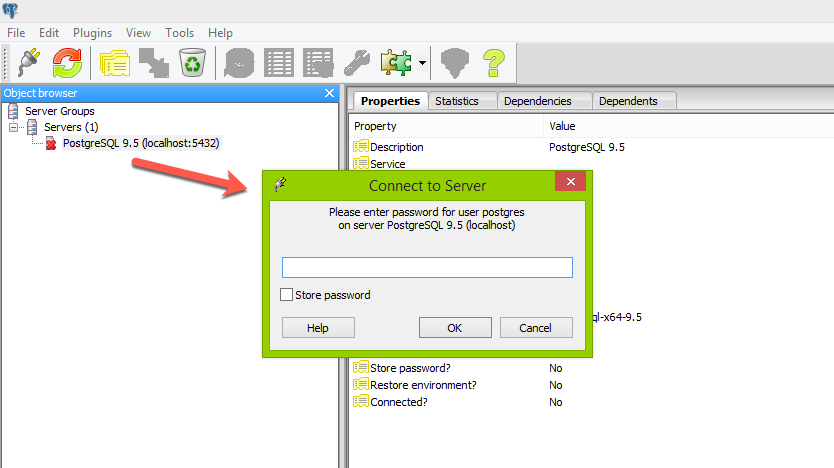
\includegraphics[width=8cm]{Images/connect_to_server.png}
	\caption{Connecting as superuser}\label{fig:connect_to_server}
\end{figure}

You can choose to store the password so you won't be asked again in the future. Once connected you will see one single database listed that is called \textit{postgres}. This is a system database that PostgreSQL needs to work properly and it cannot be modified or deleted. Under \textit{Login Roles} you should see one single role \textit{postgres}, that's the database superuser you just used to log on. Select the \textit{postgres} database and click the SQL icon in the toolbar to open an SQL query dialog (Figure \ref{fig:sql_icon}). \gls{sql} is a standard to query databases and to create and manipulate database objects (such as users, tables, etc.). In the SQL dialog you can run arbitrary SQL statements.

\begin{figure}[htb]
	\centering
	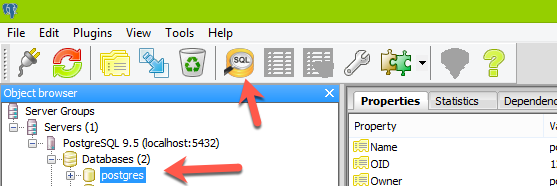
\includegraphics[width=8cm]{Images/sql_icon.png}
	\caption{Open an SQL query dialog}\label{fig:sql_icon}
\end{figure}

\subsection{Creating users and groups}

Users in PostgreSQL can have the following main privileges:

\begin{itemize}
	\item SUPERUSER: All possible privileges
	\item CREATEDB: Can create databases
	\item CREATEROLE: Can create users and groups
	\item LOGIN: Can log on to a database
\end{itemize}

A user role should have the minimum privileges required for the work that user is supposed to do. Thus, it is not a good idea to work as user \textit{postgres} all the time. Let's create another user \textit{geodb\_admin} who has the privileges to create new users, databases and to log on.

\begin{lstlisting}[caption={Creating a user},label=lst:create_user]
CREATE ROLE geodb_admin CREATEROLE CREATEDB LOGIN PASSWORD 'geodb_admin';
\end{lstlisting}

Type that statement in the SQL query dialog and hit the button with the green arrow to run/execute the statement. Statements you have already run you can comment out by putting a double-dash in front of the line. This way you ``preserve'' them but they will be ignored during query execution, e.g.

\begin{lstlisting}[caption={Commenting out an SQL statement},label=lst:comment]
--CREATE ROLE mwagner LOGIN PASSWORD 'mwagner';
\end{lstlisting}

Create another user named \textit{user\_name} (replace user\_name with your name) with the privilege to log on only. Create two groups \textit{gis\_view} and \textit{gis\_update}. A group is created by creating a role without any privilege (Listing \ref{lst:create_group}).

\begin{lstlisting}[caption={Creating groups},label=lst:create_group]
CREATE ROLE gis_view;
CREATE ROLE gis_update;
\end{lstlisting}

A user is made member of a group by granting the group to the user. Make your role \textit{user\_name} member of group \textit{gis\_update}:

\begin{lstlisting}[caption={Adding a user to a group},label=lst:add_group_member]
GRANT gis_update TO user_name;
\end{lstlisting}

Group members automatically inherit the privileges granted to the group. It is good practice to grant rights on tables, views, etc. to groups instead of individual user roles. The advantage is that when changing or revoking a privilege is required, it has to be done once only for the group and not for each individual user.

To delete a user or group role use the statement as follows:

\begin{lstlisting}[caption={Deleting a role},label=lst:del_role]
DROP ROLE role_name;
\end{lstlisting}

By the end of this exercise you should have 3 user roles (\textit{postgres}, \textit{geodb\_admin}, \textit{user\_name}) and 2 group roles (\textit{gis\_update}, \textit{gis\_view}) with role \textit{user\_name} being a member of group \textit{gis\_update}. Refresh the \textit{Group Roles} and \textit{Login Roles} in the \textit{Object Browser} in \textit{pgAdmin's} main window to verify that the group and user roles were created.

\subsection{Creating databases}

\subsubsection{Preparing a template database}

Create a database named \textit{template\_postgis} like so:

\begin{lstlisting}[caption={Creating a database},label=lst:create_db]
CREATE DATABASE template_postgis;
\end{lstlisting}

This database will serve as a template for all geodatabases you will ever create, i.e. new geodatabases will be created as copy of database \textit{template\_postgis}.
Refresh \textit{Databases} in the \textit{Object Browser} of \textit{pgAdmin's} main window to verify that the database was created. Select the new database \textit{template\_postgis} in the \textit{Object browser} and open an SQL query dialog for this database. Turn this database into a spatially enabled database by loading the PostGIS extension:

\begin{lstlisting}[caption={Creating the PostGIS extension}]
CREATE EXTENSION postgis;
\end{lstlisting}

This will add spatial capabilities to database \textit{template\_postgis}. Disallow that anyone can create tables and other database objects in schema \textit{public}:

\begin{lstlisting}[caption={Revoking a privilege}]
REVOKE CREATE ON SCHEMA public FROM public;
\end{lstlisting}

Schemas will be discussed in detail in the next chapter. For the moment just run the statement like this. Finally declare database \textit{template\_postgis} as template database. This is required for the database to serve as a template for other databases:

\begin{lstlisting}[caption={Declaring a template database}]
UPDATE pg_database SET datistemplate = true WHERE datname = 'template_postgis';
\end{lstlisting}

With this you are done setting up a template database for all geodatabases to be created in the future.
Save the SQL statements you have run so far and close the SQL query dialog. In the \textit{Object Browser} right-click on database \textit{template\_postgis} and select \textit{Disconnect database}. This is important for the database to be copied as described in the next exercise.

\subsubsection{Creating the training database}

Use the user role \textit{geodb\_admin} you created during the previous exercise to create a new database named \textit{my\_first\_geodb} based on database \textit{template\_postgis}. To run an SQL statement as \textit{geodb\_admin} you have to create a new server connection in \textit{pgAdmin} first. Click the first button in the toolbar of pgAdmin's main window and set the connection parameters as shown in Figure \ref{fig:new_server_conn}.

\begin{figure}[htb]
	\centering
	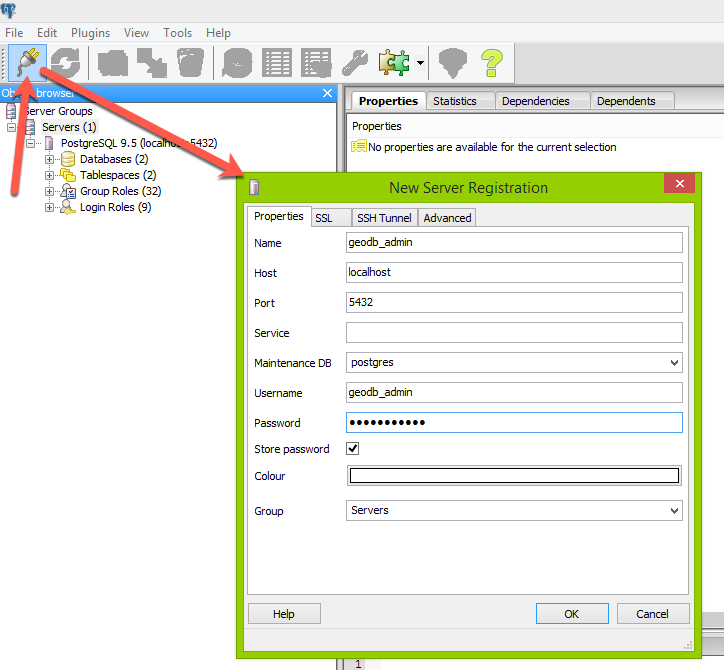
\includegraphics[width=12cm]{Images/new_server_conn.png}
	\caption{Creating a new server connection}\label{fig:new_server_conn}
\end{figure}

You will now find two server connections in the \textit{Object Browser}, one as user \textit{postgres} and one as user \textit{geodb\_admin}. Under the connection of \textit{geodb\_admin} select database \textit{postgres} in the \textit{Object Browser} and open a new SQL query dialog. Run the statement as follows to create the database \textit{my\_first\_database}:

\begin{lstlisting}[caption={Creating the training database}]
CREATE DATABASE my_first_geodb TEMPLATE = template_postgis;
\end{lstlisting}

This will create the new database as copy of \textit{template\_postgis}. Hence, \textit{my\_first\_geodb} is a geodatabase without any additional steps required. Finally grant a CREATE privilege on the database to user \textit{user\_name}:

\begin{lstlisting}[caption={Granting a CREATE privilege on a database}]
GRANT CREATE ON DATABASE my_first_geodb TO user_name;
\end{lstlisting}

This will allow the user \textit{user\_name} to create a schema in the database in a later exercise.
Deleting a database is done like so:

\begin{lstlisting}[caption={Deleting a database}]
DROP DATABASE my_db;
\end{lstlisting}

\subsection{Creating schemas}

A database may contain one or more named schemas. A schema is a bit like a folder in a file system but schemas cannot be nested. Schemas are used to:

\begin{itemize}
	\item Allow many users to use one database without interfering with each other (Two tables can have the same name if they exist in different schemas.)
	\item Organize database objects into logical groups
\end{itemize}

A schema is created like so:

\begin{lstlisting}[caption={Creating a schema}]
CREATE SCHEMA cadastre;
\end{lstlisting}

A table in a schema can be accessed by \textit{schema.table} e.g. a table \textit{parcel} in a schema \textit{cadastre}:

\begin{lstlisting}[caption={Accessing objects in a schema}]
SELECT * FROM cadastre.parcel;
\end{lstlisting}

For anyone to access any object in a schema a USAGE privilege has to be granted on that schema by the owner of the schema:

\begin{lstlisting}[caption={Granting USAGE privilege}]
GRANT USAGE ON SCHEMA cadastre TO public;
\end{lstlisting}

As user \textit{geodb\_admin} create two schemas \textit{vector\_data} and \textit{raster\_data} in database \textit{my\_first\_geodb}. To do that you have to select database \textit{my\_first\_geodb} in the \textit{Object Browser} and then open a new SQL query dialog.

\begin{lstlisting}[caption={Creating example schemas}]
CREATE SCHEMA vector_data;
CREATE SCHEMA raster_data;
\end{lstlisting}

Grant the USAGE right on both schemas to \textit{public}:

\begin{lstlisting}[caption={Granting USAGE privilege on example schemas}]
GRANT USAGE ON SCHEMA vector_data TO public;
GRANT USAGE ON SCHEMA raster_data TO public;
\end{lstlisting}

A schema and all the contained objects (tables, views, etc.) are deleted as follows:

\begin{lstlisting}[caption={Deleting a schema}]
DROP SCHEMA cadastre CASCADE;
\end{lstlisting}

\subsection{Creating tables}

Tables are created using the CREATE TABLE statement:

\begin{lstlisting}[caption={Creating a spatial table}]
CREATE TABLE vector_data.river (
gid SERIAL PRIMARY KEY,
name VARCHAR(50),
length INT,
depth DECIMAL(3, 2),
polluted BOOLEAN DEFAULT FALSE,
date_last_checked DATE
);

SELECT AddGeometryColumn('vector_data', 'river', 'geometry', 32740, 'MULTILINESTRING', 2);
\end{lstlisting}

Lines 1-8 will create a standard (i.e. not a spatial) table \textit{river} in schema \textit{vector\_data}. To add a geometry column to this table the statement in line 10 is required. The arguments to be provided to the \textit{AddGeometryColumn} functions are these:

\begin{itemize}
	\item Schema name
	\item Table name
	\item Geometry column name
	\item Spatial Reference System ID
	\item Geometry type
	\item Geometry dimension
\end{itemize}

Any time you want to add a geometry column to a table you use the statement in line 10 and adjust it accordingly.

By default only the table owner has the privilege to select, insert, update or delete data from a table. For other users to access the table's data the table owner (e.g. \textit{geodb\_admin}) has to grant the required privileges:

\begin{lstlisting}[caption={Granting privileges on table and sequence}]
GRANT SELECT, INSERT, UPDATE, DELETE ON TABLE vector_data.river TO gis_update;
GRANT SELECT ON TABLE vector_data.river TO gis_view;
GRANT USAGE ON SEQUENCE vector_data.river_gid_seq TO gis_update;
\end{lstlisting}

In line 1 full access is granted to group \textit{gis\_update} (and to anyone being a member). In line 2 a SELECT privilege is granted to group \textit{gis\_view} (and to anyone being a member). In line 3 a USAGE privilege is granted to group \textit{gis\_update} on a sequence. The \textit{river} table's primary key is a serial number i.e. a number that is automatically advanced by 1 every time a new row is inserted into the table. PostgreSQL creates a so called sequence for each serial number that requires a USAGE privilege to be used (i.e. to be advanced). The final thing you will want to do is to create a spatial index on the geometry column. This will speed up spatial queries involving this table significantly:

\begin{lstlisting}[caption={Creating a spatial index}]
CREATE INDEX river_geometry_idx ON vector_data.river USING gist(geometry);
\end{lstlisting}

A table is deleted as follows:

\begin{lstlisting}[caption={Deleting a schema}]
DROP TABLE vector_data.river;
\end{lstlisting}

Create the \textit{river} table, grant the privileges and create the spatial index. Launch QGIS and load the \textit{district} Shapefile from the \textit{Data/Shapefiles} folder. Now load the \textit{river} table from your database. You will have to create a new connection to a PostgreSQL/PostGIS database first (Figure \ref{fig:postgis_conn}). Use your username as the username to connect. 

\begin{figure}[htb]
	\centering
	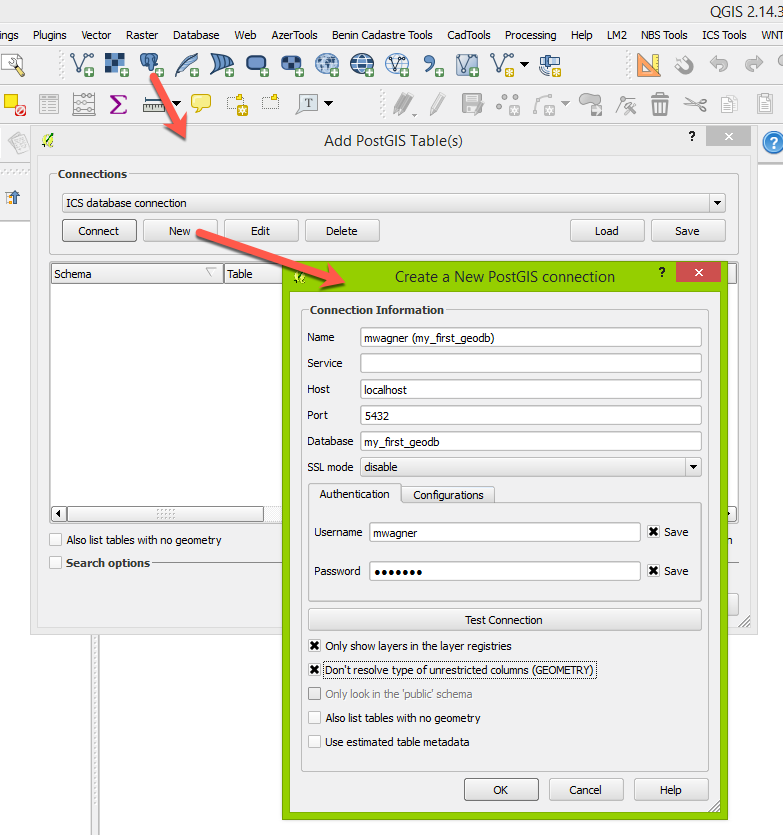
\includegraphics[width=12cm]{Images/postgis_conn.png}
	\caption{Connecting to PostgreSQL from within QGIS}\label{fig:postgis_conn}
\end{figure}

In the \textit{Add PostGIS Table(s)} dialog click the \textit{Connect} button, you should see the \textit{river} table you previously created under schema \textit{vector\_data} (Figure \ref{fig:postgis_conn2}). Select and add the table to QGIS. Toggle editing and digitise ten fictive rivers on Mahe. Set the \textit{polluted} field to true for some of the rivers. Save your changes. Use the \textit{Field Calculator} to populate the \textit{length} field of the river table. Again, save your changes.

\begin{figure}[htb]
	\centering
	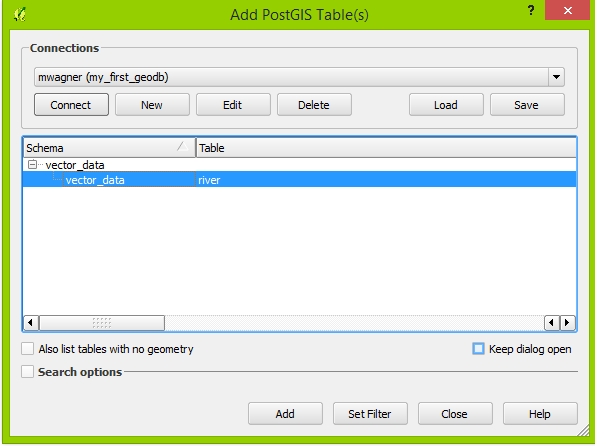
\includegraphics[width=8cm]{Images/postgis_conn2.png}
	\caption{List of spatial tables}\label{fig:postgis_conn2}
\end{figure}

\subsection{Creating views}

You can create views over queries you need to run frequently to:

\begin{itemize}
	\item Avoid typing the query each time the query is needed
	\item Give a name to the query
\end{itemize}

If the view contains a geometry column it becomes a spatial view that can be loaded and visualised in QGIS, e.g.:

\begin{lstlisting}[caption={Creating a view}]
CREATE OR REPLACE VIEW polluted_rivers AS SELECT * FROM vector_data.river WHERE polluted = true;
\end{lstlisting}

As with the tables the required privileges have to be granted on the view for other users to access the view:

\begin{lstlisting}[caption={Granting privileges on spatial view}]
GRANT SELECT ON VIEW vector_data.polluted_rivers TO gis_update, gis_view;
\end{lstlisting}

Create the view \textit{polluted\_rivers} as \textit{geodb\_admin} and grant the privileges for others to SELECT from the view.

\section{Importing spatial data}

PostGIS supports the storage and analysis of vector and raster data.

\subsection{Importing vector data}

There is a number of tools to import vector data into a PostgreSQL/PostGIS database but we will use the \textit{PostGIS Shapefile and DBF Loader} that came with the PostGIS installation. Find and launch the tool and enter the database connection parameters (Figure \ref{fig:load_shapefiles1}).

\begin{figure}[htb]
	\centering
	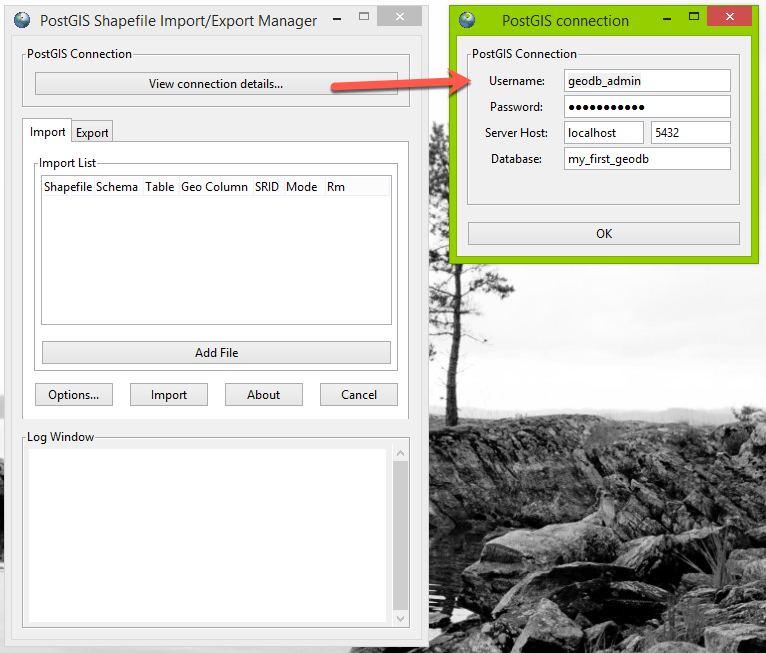
\includegraphics[width=8cm]{Images/load_shapefiles1.png}
	\caption{Setting the database connection parameters for the Loader}\label{fig:load_shapefiles1}
\end{figure}

Click the \textit{Add File} button and select all Shapefiles from the \textit{Data/Shapefiles} folder except of the \textit{river} file (you already have a \textit{river} table). You can select multiple Shapefiles at once. The Loader tries to import the data from the Shapefiles into schema \textit{public} by default. We don't want that, they should go in schema \textit{vector\_data}. Double-click in the \textit{Schema} field of each table and change the schema from \textit{public} to \textit{vector\_data}. The SRID is 0 by default, we have to change that to 32740. Again do that for each table entry. Finally we want to change the name of column that will hold the geometry from \textit{geom} to \textit{geometry} (Figure \ref{fig:load_shapefiles2}).

\begin{figure}[htb]
	\centering
	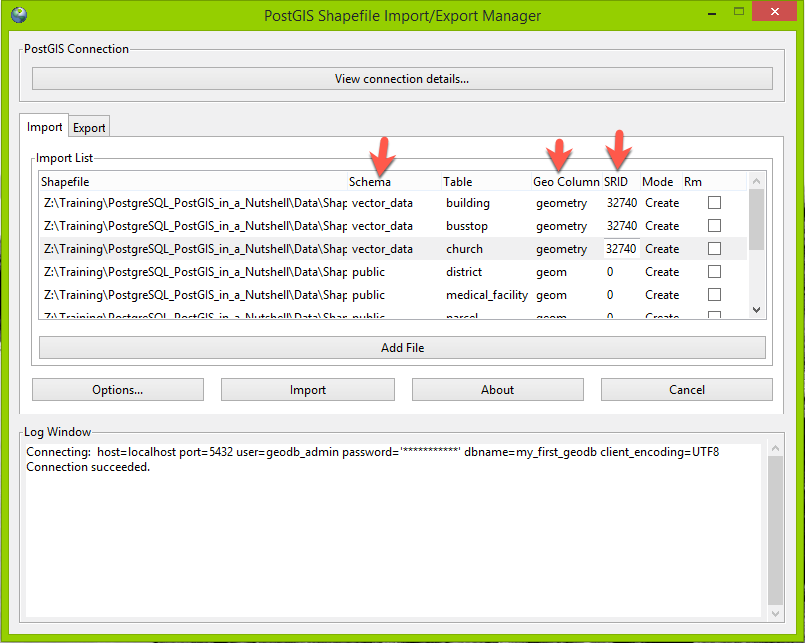
\includegraphics[width=8cm]{Images/load_shapefiles2.png}
	\caption{Correcting the import settings}\label{fig:load_shapefiles2}
\end{figure}

Once all preparation has been done click the \textit{Import} button. The import might take a few seconds. Once finished refresh the \textit{Object Browser} in \textit{pgAdmin} and verify that the new tables are there. You should find 11 tables now in schema \textit{vector\_data}. During the import spatial indices were created automatically for all new tables. What is still missing is to grant the privileges for other users to be able to access the new tables. You have to grant the same privileges on each new table and sequence that you previously granted on table river and the relating sequence. You can copy and paste these statements and just modify table and sequence name. This step has to be done by \textit{geodb\_admin}, the owner of all tables.

After granting the required privileges you can load the new tables into QGIS.

\subsection{Importing raster data}

Importing raster data has to be done via command prompt, no graphical tool is yet provided for raster import. Open a Command Prompt by typing \textit{cmd} in the Windows Search. Open the Windows File Explorer and navigate to the \textit{bin} directory of your PostgreSQL installation. Copy that path from the address bar. In the Command Prompt type \textit{cd} (change directory) and paste the path you just copied from the File Explorer. It should look similar to Listing \ref{lst:cmd}. Hit Enter.

\begin{lstlisting}[caption={Changing directory},label=lst:cmd]
cd "C:\Program Files\PostgreSQL\9.5\bin
\end{lstlisting}

Changing the directory is required for the raster data import tool (\textit{raster2pgsql}) to be found. Finally type:

\begin{lstlisting}[caption={Importing raster data into the database}]
raster2pgsql -I -C -e -Y -F -s 32740 -t auto -l 2,4,8,16,32,64 Z:\PostgreSQL_PostGIS_in_a_Nutshell\Data\DEM\Mahe_DEM.tif raster_data.mahe_dem | psql -U geodb_admin -d my_first_geodb
\end{lstlisting}

Change the path to your DEM file as required end hit Enter. The import might take several minutes depending on your computer's performance.
As a result you will find seven new tables in schema \textit{raster\_data}. The first one is the main table with the raster data in original resolution (\textit{mahe\_dem}). The other tables are overview levels of the original raster with lower resolutions. They will make loading the raster data in QGIS significantly faster. As for the parameters used with the import tool check the PostGIS documentation for a detailed description. Similar to the vector data tables the raster data tables cannot be accessed by other users yet directly after the import. You have to grant the required privileges first as \textit{geodb\_admin}: 

\begin{lstlisting}[caption={Granting privileges on raster tables}]
GRANT SELECT ON raster_data.mahe_dem TO gis_update, gis_view;
GRANT SELECT ON raster_data.o_2_mahe_dem TO gis_update, gis_view;
GRANT SELECT ON raster_data.o_4_mahe_dem TO gis_update, gis_view;
GRANT SELECT ON raster_data.o_8_mahe_dem TO gis_update, gis_view;
GRANT SELECT ON raster_data.o_16_mahe_dem TO gis_update, gis_view;
GRANT SELECT ON raster_data.o_32_mahe_dem TO gis_update, gis_view;
GRANT SELECT ON raster_data.o_64_mahe_dem TO gis_update, gis_view;
\end{lstlisting}

A read-only (SELECT) privilege should be sufficient for the raster data tables since it is unlikely that these tables need modification.
In QGIS open the \textit{DB Manager} from the \textit{Database} menu. Under \textit{PostGIS} find your connection and navigate to schema \textit{raster\_data}. Drag and drop table \textit{mahe\_dem} in the QGIS map window (Figure \ref{fig:add_pg_raster}).
 
\begin{figure}[htb]
	\centering
	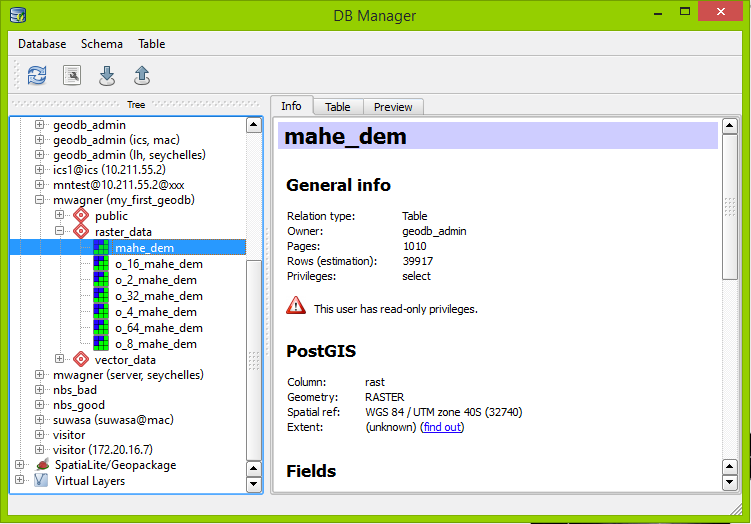
\includegraphics[width=8cm]{Images/add_pg_raster.png}
	\caption{Add a PostGIS raster layer}\label{fig:add_pg_raster}
\end{figure}

\section{Spatial analysis}

Let the fun begin. As user \textit{user\_name} create a schema named \textit{user\_name}. Any views you will create during this exercise you create in that schema. Before creating the schema you need to create a new server connection in \textit{pgAdmin} for user \textit{user\_name}. Then select database \textit{my\_first\_geodb} and open a new SQL query dialog. Create the schema and then run the queries as follows: 

\begin{itemize}
	\item List parcel number, gid and description of all parcels with invalid geometry.
\begin{lstlisting}
SELECT id AS parcel_no, gid, ST_IsValidReason(geometry) AS reason FROM vector_data.parcel WHERE NOT ST_IsValid(geometry);
\end{lstlisting}
	\item List gid and geometry as GeoJSON for the first 3 buildings.
\begin{lstlisting}
SELECT gid, ST_AsGeoJSON(geometry, 1) FROM vector_data.building LIMIT 3;
\end{lstlisting}
	\item List parcel number and area of the 5 largest parcels.
\begin{lstlisting}
SELECT id, ST_Area(geometry) AS area_m2 FROM vector_data.parcel ORDER BY area_m2 DESC LIMIT 5;
\end{lstlisting}
	\item List parcel number and geometry (as plain text) of the 3 smallest parcels.
\begin{lstlisting}
SELECT id, ST_AsText(geometry) FROM vector_data.parcel ORDER BY ST_Area(geometry) LIMIT 3;
\end{lstlisting}
	\item How many parcels are crossed by a river?
\begin{lstlisting}
SELECT count(a.*) FROM vector_data.parcel a, vector_data.river b WHERE ST_Intersects(a.geometry, b.geometry);
\end{lstlisting}
	\item Find all donut buildings (buildings with holes) and create a spatial view to visualise them in QGIS.
\begin{lstlisting}
CREATE OR REPLACE VIEW user_name.donut_buildings AS SELECT * FROM vector_data.building WHERE ST_NRings(geometry) > 1;
\end{lstlisting}
	\item List the church name and terrain elevation at each churches location.
\begin{lstlisting}
SELECT b.name as church_name, round(st_value(a.rast, b.geometry)) AS elevation FROM raster_data.mahe_dem a, vector_data.church b WHERE ST_Intersects(a.rast, b.geometry) ORDER BY elevation;
\end{lstlisting}
	\item Show the number of parcels per district.
\begin{lstlisting}
SELECT a.name as district_name, count(b.*) as parcel_count FROM vector_data.district a, vector_data.parcel b WHERE ST_Intersects(a.geometry, b.geometry) group by a.name ORDER BY a.name;
\end{lstlisting}
\end{itemize}

Based on the SQL statements for the example queries try to solve the tasks as follows:

\begin{enumerate}
	\item Of the rivers you created find the three longest ones.
	\item Find the police station with the largest distance to any health care facility.
	\item Create a spatial view to show all buildings built over a parcel's boundary.
	\item What's the total length of road segments within Anse Royale (in km)?
	\item Create a spatial view for a 500m buffer around each health care facility.
	\item Find the schools that have no busstop within 200m?
\end{enumerate}

Make use the PostGIS reference manual that you will find in the \textit{Software} folder.

\end{document}
